% ======================================================================
% BLOQUE 2 — Rayos cósmicos y astrofísica de altas energías
% ======================================================================
\section{Rayos cósmicos}
\bloque{RAYOS CÓSMICOS}

% ---------------------------------------------------------------- 16
\begin{frame}{Rayos cósmicos: aceleradores naturales}
  \begin{columns}[c,onlytextwidth]
    \column{0.45\textwidth}
      \small
      Descubiertos por V.~Hess en 1912. Los primarios cargados son
      \textbf{núcleos}: $\sim$90\% protones, $\sim$9\% helio, $\sim$1\% más
      pesados, con energías de hasta \textbf{más de $10^{20}$\,eV}.
      \vspace{6pt}

      \centering
      \begin{tikzpicture}[x=1cm,y=1cm]
        \shade[ball color=itedaOrange!70] (0,0) circle (0.25);
        \node[font=\tiny, below=3pt] at (0,-0.25) {fuente};
        \draw[very thick, itedaOrange, -{Stealth}] (0.3,0.05)
          .. controls (1.4,1.2) and (2.0,-1.0) .. (3.0,0.2)
          .. controls (3.6,0.9) and (4.0,0.0) .. (4.6,-0.1);
        \draw[dashed, itedaGray] (0.3,0) -- (4.6,0);
        \shade[ball color=cmbAzul!60] (4.85,-0.1) circle (0.22);
        \node[font=\tiny, below=3pt] at (4.85,-0.32) {Tierra};
        \draw[thick, itedaTealDark, -{Stealth}] (4.6,-0.1) -- ++(-0.9,0.75)
          node[above, font=\tiny, align=center] {dirección\\aparente};
      \end{tikzpicture}\\[4pt]
      \begin{clave}
        Los campos magnéticos de la galaxia y del espacio intergaláctico
        curvan su trayectoria: la dirección de llegada \textbf{no apunta} a la
        fuente.
      \end{clave}
    \column{0.52\textwidth}
      \centering
      \begin{tikzpicture}[x=1cm,y=1cm]
        \tikzset{tarjeta/.style={rounded corners=3pt, minimum width=6.9cm,
          inner sep=4pt, text width=6.6cm, align=left, font=\footnotesize}}
        \node[tarjeta, fill=itedaOrange!15, draw=itedaOrange] at (0,3.2)
          {\textbf{\color{itedaOrange}Núcleos cargados}: llegan muchos, pero
          \textbf{desviados} por campos magnéticos y frenados por los fondos
          de radiación.};
        \node[tarjeta, fill=cmbAzul!12, draw=cmbAzul] at (0,1.6)
          {\textbf{\color{cmbAzul}Fotones gamma}: viajan en línea recta, pero se
          \textbf{absorben} ($\gamma\gamma\to e^+e^-$). A PeV, el horizonte es
          la galaxia.};
        \node[tarjeta, fill=violetaNu!12, draw=violetaNu] at (0,0)
          {\textbf{\color{violetaNu}Neutrinos}: ni se desvían ni se absorben,
          pero casi \textbf{no interactúan}.};
      \end{tikzpicture}
  \end{columns}
\end{frame}

% ---------------------------------------------------------------- 17
\begin{frame}{El espectro de los rayos cósmicos}
  \begin{columns}[c,onlytextwidth]
    \column{0.50\textwidth}
      \centering
      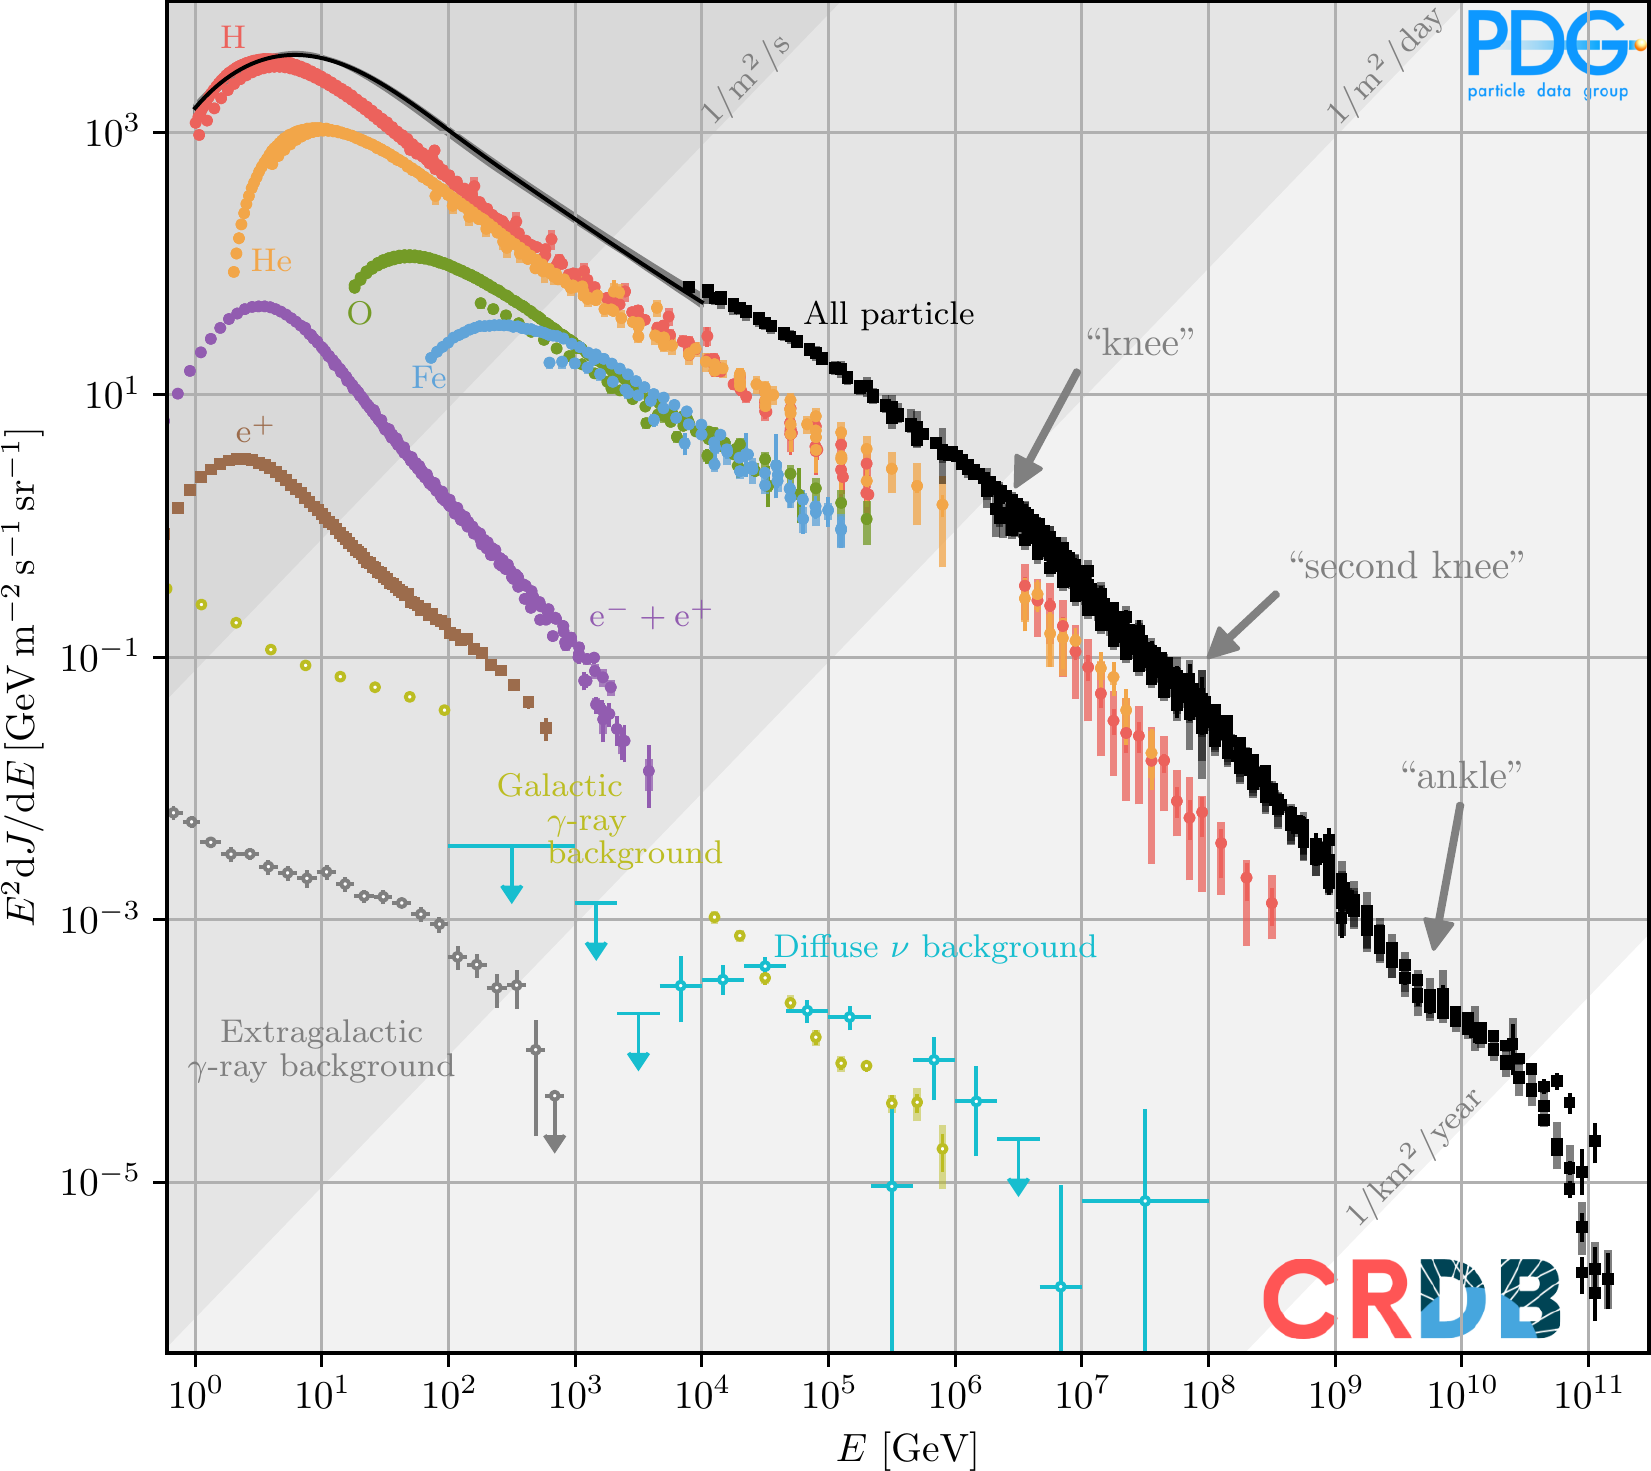
\includegraphics[width=\linewidth]{externas/pdg2024_espectro_E2.png}
    \column{0.47\textwidth}
      \small
      El flujo cae como $E^{-2,7}$: lo que se ve es el flujo
      \textbf{multiplicado por $E^2$}. Las diagonales grises marcan cuántas
      partículas llegan por encima de esa energía:\\[4pt]
      \begin{tikzpicture}
        \foreach \y/\e/\f in {0/{$10^{11}$ eV}/{1 partícula por m$^2$ por segundo},
            -0.5/{$\sim3\times10^{15}$ eV}/{1 por m$^2$ por año (\emph{rodilla})},
            -1.0/{$\sim10^{19}$ eV}/{$\sim$1 por km$^2$ por año},
            -1.5/{$\sim5\times10^{19}$ eV}/{$\sim$1 por km$^2$ por \textbf{siglo}}}{
          \node[anchor=west, text=itedaOrange, font=\footnotesize\bfseries] at (0,\y) {\e};
          \node[anchor=west, font=\footnotesize] at (2.45,\y) {\f};}
      \end{tikzpicture}\\[2pt]
      \begin{clave}
        \textbf{Colores}: hasta $\sim$100\,TeV se mide cada núcleo
        directamente, con satélites y globos. \textbf{Negro}: por encima,
        sólo con \textbf{lluvias atmosféricas extensas}.
      \end{clave}
  \end{columns}
  \credito{Figura: Particle Data Group, \textit{Review of Particle Physics} (2024), Fig.~30.1 (datos de CRDB)}
\end{frame}

% ---------------------------------------------------------------- 18
\begin{frame}{El espectro como mapa de la física}
  \centering
  \begin{tikzpicture}
    \begin{loglogaxis}[coloquio, name=arriba, scale only axis, width=12.4cm, height=3.3cm,
      xmin=1e9, xmax=3e20, ymin=0.002, ymax=80,
      ylabel={$E^{2{,}6}J$ (u.\ arb.)}, xticklabels={}, ytick=\empty,
      axis x line*=bottom, axis y line*=left]
      % Ley de potencia quebrada (pendiente = 2,6 - gamma), forma esquemática
      \addplot[very thick, itedaTeal, domain=9:15.5, samples=2]
        ({10^x},{10^(-0.1*(x-15.5))});
      \addplot[very thick, itedaTeal, domain=15.5:17, samples=2]
        ({10^x},{10^(-0.5*(x-15.5))});
      \addplot[very thick, itedaTeal, domain=17:18.7, samples=2]
        ({10^x},{10^(-0.75-0.7*(x-17))});
      \addplot[very thick, itedaTeal, domain=18.7:19.11, samples=2]
        ({10^x},{10^(-1.94+0.1*(x-18.7))});
      \addplot[very thick, itedaTeal, domain=19.11:19.66, samples=2]
        ({10^x},{10^(-1.899-0.45*(x-19.11))});
      \addplot[very thick, itedaTeal, domain=19.66:20.2, samples=20]
        ({10^x},{10^(-2.146-2.5*(x-19.66))});
      \node[font=\scriptsize\bfseries, text=itedaOrange, anchor=north east] at (axis cs:3e15,0.9) {rodilla};
      \node[font=\scriptsize\bfseries, text=itedaOrange, anchor=south west] at (axis cs:1e17,0.25) {segunda rodilla};
      \node[font=\scriptsize\bfseries, text=itedaOrange, anchor=north east] at (axis cs:4.5e18,0.0112) {tobillo};
      \node[font=\scriptsize\bfseries, text=itedaOrange, anchor=south west] at (axis cs:4e19,0.012) {supresión};
      \fill[cmbAzul!18] (axis cs:1e9,8) rectangle (axis cs:1e17,55);
      \node[font=\scriptsize, text=cmbAzul!70!black] at (axis cs:3e12,21)
        {\textbf{galácticas}: remanentes de supernova};
      \fill[pattern=north east lines, pattern color=itedaGray!70] (axis cs:1e17,8)
        rectangle (axis cs:5e18,55);
      \node[font=\scriptsize, text=itedaTealDark, fill=white, inner sep=1pt] at (axis cs:7e17,21)
        {transición};
      \fill[itedaOrange!20] (axis cs:5e18,8) rectangle (axis cs:3e20,55);
      \node[font=\scriptsize\bfseries, text=itedaOrange!70!black] at (axis cs:4e19,21)
        {extragalácticas};
      \node[font=\tiny, text=itedaGray, anchor=south west] at (axis cs:2e9,0.004)
        {$E_\mathrm{rodilla}(Z)\approx Z\,E_\mathrm{rodilla}(p)$: protones en la rodilla, hierro en la segunda};
    \end{loglogaxis}
    \begin{semilogxaxis}[coloquio, at={(arriba.south west)}, anchor=north west,
      yshift=-0.15cm, scale only axis, width=12.4cm, height=1.75cm,
      xmin=1e9, xmax=3e20, ymin=0, ymax=4.2, ytick=\empty,
      xlabel={energía $E$ [eV]}, axis y line=none, axis x line*=bottom,
      xtick={1e9,1e11,1e13,1e15,1e17,1e19}]
      \fill[itedaTeal!75, rounded corners=2pt] (axis cs:1e9,3.2) rectangle (axis cs:1e14,4.1);
      \node[font=\tiny\bfseries, text=white] at (axis cs:1e11,3.65) {satélites y globos (AMS-02, DAMPE, CALET)};
      \fill[itedaTeal!60, rounded corners=2pt] (axis cs:1e13,2.1) rectangle (axis cs:1e17,3.0);
      \node[font=\tiny\bfseries, text=white] at (axis cs:1e15,2.55) {LHAASO, IceTop, KASCADE};
      \fill[itedaTeal!45, rounded corners=2pt] (axis cs:1e16,1.0) rectangle (axis cs:3e18,1.9);
      \node[font=\tiny\bfseries, text=itedaTealDark, anchor=east] at (axis cs:9e15,1.45)
        {KASCADE-Grande, TALE, Auger (AMIGA, HEAT)};
      \fill[itedaOrange, rounded corners=2pt] (axis cs:1e18,0.0) rectangle (axis cs:3e20,0.9);
      \node[font=\tiny\bfseries, text=white] at (axis cs:1.7e19,0.45) {Pierre Auger, TA};
      \draw[dashed, cmbRojo, thick] (axis cs:1e17,0) -- (axis cs:1e17,4.2);
      \node[font=\tiny, text=cmbRojo, anchor=west] at (axis cs:1.2e17,3.65)
        {$\sqrt{s}$ del LHC $\equiv E_\mathrm{lab}\approx10^{17}$\,eV};
    \end{semilogxaxis}
  \end{tikzpicture}
  \begin{tikzpicture}[remember picture, overlay]
    \node[anchor=north east] at ([xshift=-0.3cm, yshift=-1.1cm]current page.north east)
      {\esquematico};
  \end{tikzpicture}
  \creditoizq{Pendientes: Auger, PRL 125 (2020) 121106, y compilaciones del PDG. Rangos de los experimentos aproximados.}
\end{frame}

% ---------------------------------------------------------------- 19
\begin{frame}{Zoom en ultra alta energía}
  \begin{columns}[c,onlytextwidth]
    \column{0.60\textwidth}
      \centering
      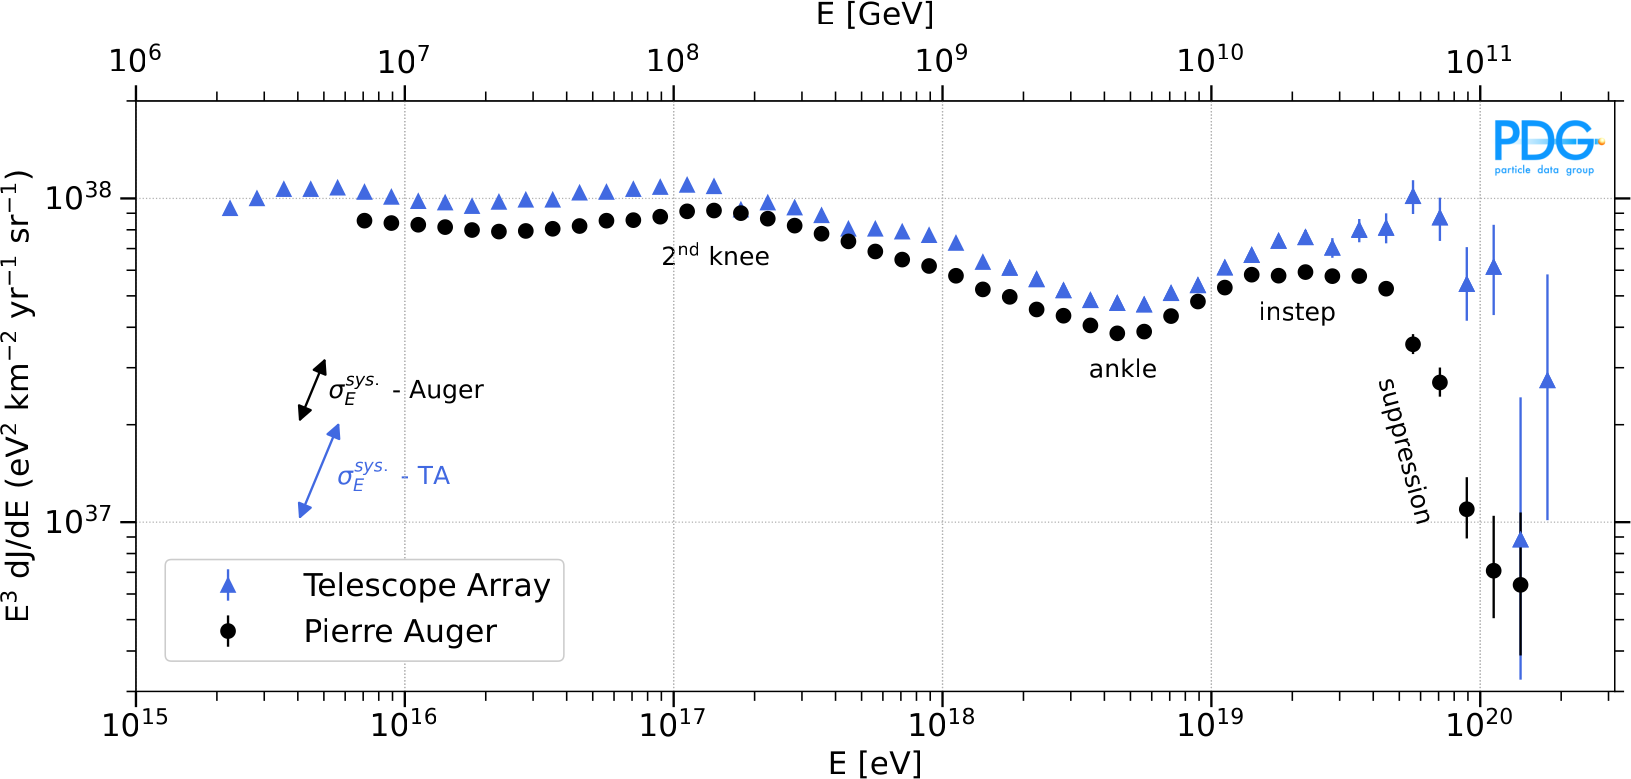
\includegraphics[width=\linewidth]{tesis/espectro_uhecr_recortado.png}
    \column{0.37\textwidth}
      \small
      Auger (2020), ley de potencia quebrada:\\[4pt]
      {\footnotesize
      \begin{tabular}{@{}lr@{}}
        \toprule
        tobillo & $E_{12}=5{,}0$\,EeV \\
        \emph{instep} & $E_{23}=13$\,EeV \\
        supresión & $E_{34}=46$\,EeV \\
        \midrule
        $\gamma_1\to\gamma_2$ & $3{,}29\to2{,}51$\\
        $\gamma_3\to\gamma_4$ & $3{,}05\to5{,}1$\\
        \bottomrule
      \end{tabular}}\\[6pt]
      \begin{clave}
        Supresión a más de 20$\sigma$. ¿Propagación o límite de las fuentes?
        El espectro solo no alcanza.
      \end{clave}
  \end{columns}
  \credito{Figura: PDG (2024), datos de Pierre Auger y Telescope Array}
\end{frame}

% ---------------------------------------------------------------- 19
\begin{frame}{Cómo se acelera: el mecanismo de Fermi en choques}
  \begin{columns}[c,onlytextwidth]
    \column{0.46\textwidth}
      \centering
      \begin{tikzpicture}[x=1cm,y=1cm]
        \fill[itedaOrange!10] (-3,-1.6) rectangle (0,1.9);
        \fill[cmbAzul!10] (0,-1.6) rectangle (3,1.9);
        \draw[itedaOrange, line width=2pt] (0,-1.6) -- (0,1.9);
        \node[font=\scriptsize, align=center] at (-1.5,1.55) {gas ya chocado};
        \node[font=\scriptsize, align=center] at (1.5,1.55) {gas en reposo};
        \draw[flecha, itedaOrange] (-0.6,-1.25) -- (0.6,-1.25)
          node[right, font=\tiny, text=itedaTealDark] {el choque avanza};
        \draw[very thick, violetaNu, -{Stealth}, rounded corners=4pt]
          (-2.3,-0.4) -- (-1.2,0.2) -- (-0.4,-0.3) -- (0.9,0.5) -- (2.2,0.1)
          -- (1.2,0.9) -- (-0.7,0.6) -- (-1.6,1.0) -- (-0.3,0.95) -- (1.7,0.75);
        \foreach \x/\y in {-2.2/0.7,-1.4/-0.8,-0.6/1.2,0.8/-0.6,1.6/1.1,2.4/-0.3}{
          \draw[itedaGray!70, decorate, decoration={coil, aspect=0.4, segment length=1.6mm, amplitude=0.9mm}]
            (\x-0.25,\y) -- (\x+0.25,\y);}
        \node[font=\scriptsize, text=violetaNu] at (2.35,0.95) {$E\uparrow$};
      \end{tikzpicture}\\[4pt]
      {\scriptsize Espirales grises: irregularidades del campo magnético que
      actúan como «espejos».}
    \column{0.51\textwidth}
      \footnotesize
      \begin{enumerate}\footnotesize
        \item Una supernova lanza una \textbf{onda de choque} a miles de km/s.
        \item Campos magnéticos \textbf{turbulentos} a ambos lados hacen
          rebotar a la partícula, que cruza el choque una y otra vez.
        \item En cada cruce el gas del otro lado \textbf{viene hacia ella},
          como una pelota entre dos raquetas que se acercan: gana $\sim$1\% de
          energía.
        \item En cada vuelta puede \textbf{escaparse} y dejar de acelerarse.
      \end{enumerate}
      \begin{clave}
        Muchas ganan poco y pocas muchísimo: una \textbf{ley de potencia}
        $E^{-2}$ ($E^{-2,7}$ tras escapar de la galaxia).
      \end{clave}
  \end{columns}
\end{frame}

% ---------------------------------------------------------------- 20
\begin{frame}{Criterio de Hillas: ¿quién llega a $10^{20}$ eV?}
  \begin{columns}[c,onlytextwidth]
    \column{0.52\textwidth}
      \centering
      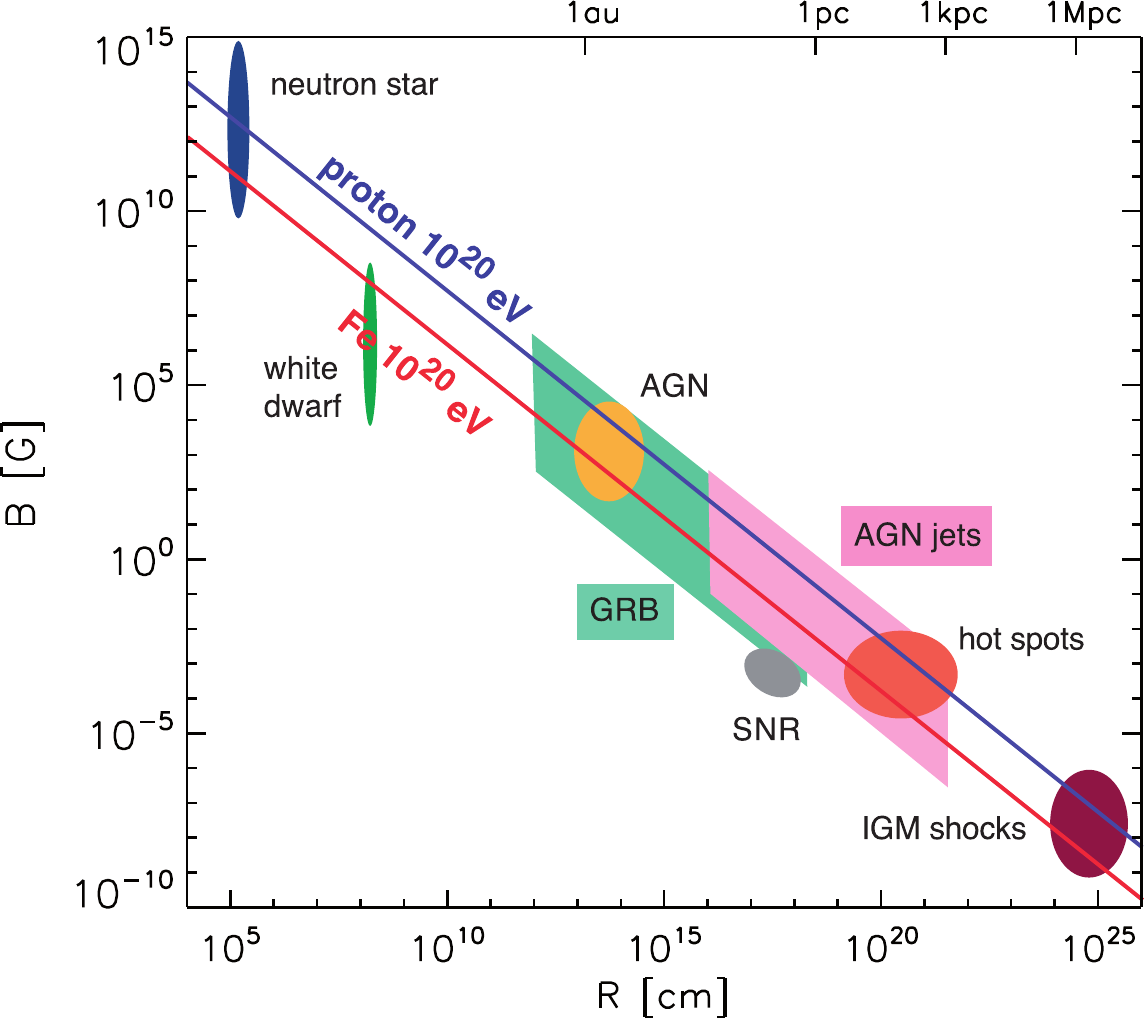
\includegraphics[width=\linewidth]{externas/hillas_aloisio2017.png}
    \column{0.45\textwidth}
      \small
      Para seguir ganando energía, la partícula tiene que quedar
      \textbf{atrapada} girando en la región que la acelera: su radio de giro
      debe ser menor que el tamaño de la fuente.
      \vspace{2pt}
      \begin{clave}
        \centering
        $E_\mathrm{max}\;\approx\;Z\;\beta\;B\;R$
      \end{clave}
      \vspace{2pt}
      {\footnotesize $Z$: carga del núcleo (el hierro llega 26 veces más
      lejos) · $\beta$: velocidad del choque · $B$: campo magnético · $R$:
      tamaño.}\\[4pt]
      {\footnotesize Sobre las diagonales se llega a $10^{20}$\,eV: campos
      enormes en objetos chicos o débiles en regiones gigantes. Necesario, no
      suficiente.}
  \end{columns}
  \creditoizq{Figura: Kotera \& Olinto, ARA\&A 49 (2011) 119, vía Aloisio, PTEP 2017 12A102 (Fig.~12)}
\end{frame}

% ---------------------------------------------------------------- 22
\begin{frame}{El viaje no es gratis: efecto GZK y fotodesintegración}
  \begin{columns}[c,onlytextwidth]
    \column{0.52\textwidth}
      \centering
      \begin{tikzpicture}[x=1cm,y=1cm]
        \node[font=\small\bfseries] (p) at (0,0) {$p$};
        \node[font=\small, text=cmbAzul] (g) at (0,-1.4) {$\gamma_\mathrm{CMB}$};
        \node[circle, fill=itedaOrange!25, draw=itedaOrange, font=\small, inner sep=1pt]
          (D) at (1.6,-0.7) {$\Delta^+$};
        \draw[flecha] (p) -- (D);
        \draw[foton, cmbAzul] (g) -- (D);
        \node[font=\small, anchor=west] (n) at (2.8,0.2) {$n\,\pi^+$};
        \node[font=\small, anchor=west] (pp) at (2.8,-1.6) {$p\,\pi^0$};
        \draw[flecha] (D) -- (n.west);
        \draw[flecha] (D) -- (pp.west);
        \node[font=\small, text=violetaNu, anchor=west] at (3.6,0.2)
          {$\to\mu^+\nu_\mu\to e^+\nu_e\bar\nu_\mu\nu_\mu$};
        \node[font=\small, text=cmbAzul, anchor=west] at (3.6,-1.6) {$\to\gamma\gamma$};
        \node[font=\scriptsize, text=violetaNu, anchor=north] at (5.0,-0.1)
          {neutrinos \textbf{cosmogénicos}};
      \end{tikzpicture}\\[6pt]
      \small
      \[ E_\mathrm{th}=\frac{m_\pi\,(2m_p+m_\pi)}{4\varepsilon}\approx10^{20}\,\mathrm{eV}
         \quad (\varepsilon\approx6\times10^{-4}\,\mathrm{eV}) \]
      {\footnotesize La cola de Planck lo baja a $\sim5\times10^{19}$\,eV.
      Pierde $\sim$20\% por interacción: horizonte de $\sim$50--100\,Mpc.}
    \column{0.45\textwidth}
      \small
      \begin{itemize}\footnotesize
        \item \textbf{Protones}: piones (GZK, 1966) y pares $e^+e^-$.
        \item \textbf{Núcleos}: fotodesintegración en el CMB y el fondo
          infrarrojo; umbral $\propto A$.
        \item \textbf{Fuentes}: energía máxima $E_\mathrm{max}\propto Z$.
      \end{itemize}
      \begin{clave}
        Los escenarios \textbf{no se excluyen}. Separarlos requiere
        \textbf{espectro, composición y anisotropías}.
      \end{clave}
  \end{columns}
\end{frame}

% ---------------------------------------------------------------- 23
\begin{frame}{Composición y direcciones de llegada}
  \begin{columns}[T,onlytextwidth]
    \column{0.50\textwidth}
      \centering
      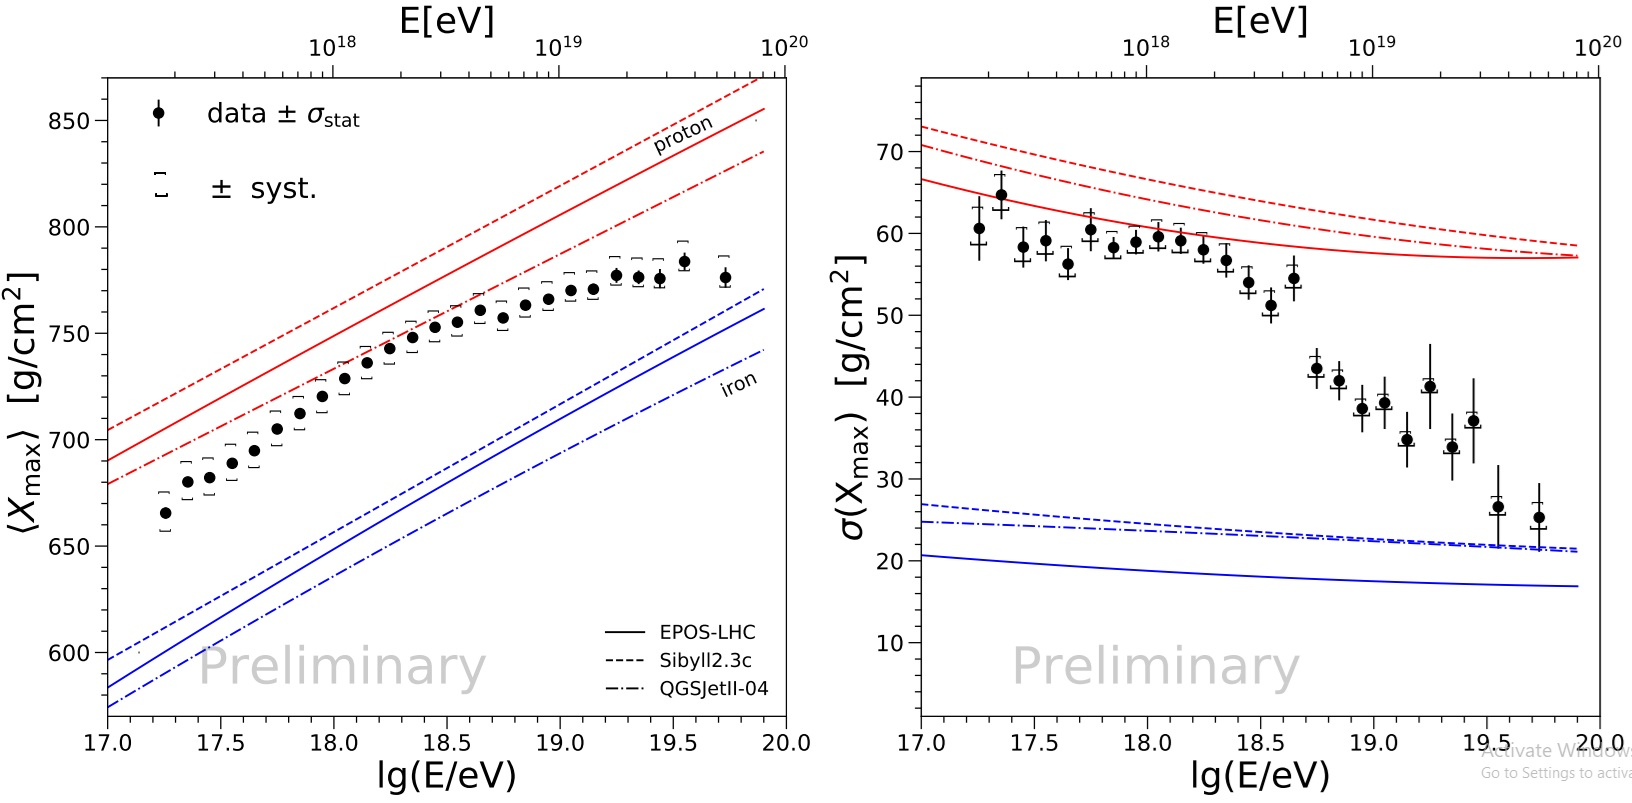
\includegraphics[width=\linewidth]{tesis/x_max.jpg}\\[3pt]
      {\footnotesize $\langle X_\mathrm{max}\rangle$ y $\sigma(X_\mathrm{max})$ se
      alejan de protón: composición \textbf{más pesada} por encima de
      $\sim$3\,EeV.}
    \column{0.47\textwidth}
      \centering
      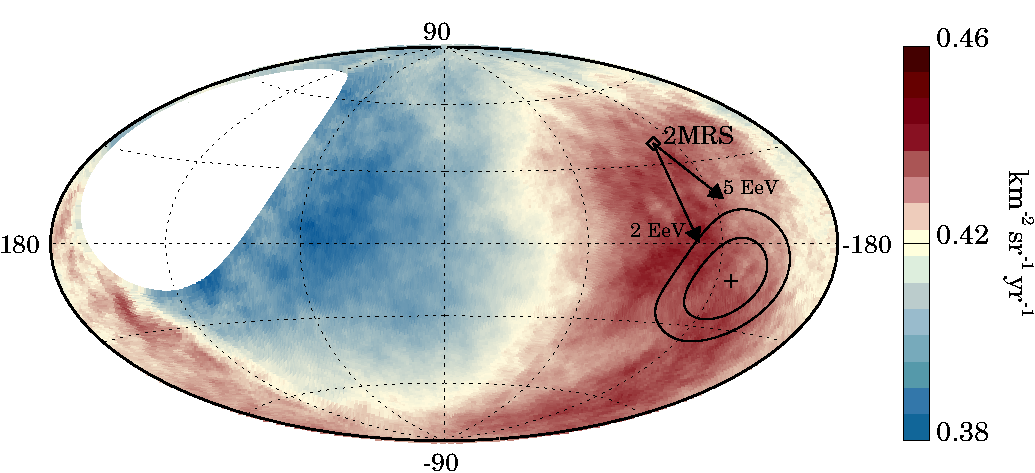
\includegraphics[width=0.9\linewidth]{externas/auger_dipolo_galactico_2017.pdf}\\[2pt]
      {\footnotesize Por encima de 8\,EeV: un \textbf{dipolo} de $\sim$7\% lejos
      del centro galáctico ($>6\sigma$): \textbf{origen extragaláctico}.}\\[4pt]
      \begin{clave}
        Favorece fuentes de \textbf{rigidez máxima limitada} y composición
        mixta (según el modelo hadrónico).
      \end{clave}
  \end{columns}
  \creditoizq{Izq.: Auger (A.~Yushkov), ICRC 2019. Der.: Auger, Science 357 (2017) 1266; significancia: ICRC 2025}
\end{frame}
